%=====================================================================
%  DataScience_Fall2026_CourseAtAGlance.tex
%
%  Standalone one-page export of the "Course at a Glance" diagram
%  (fig:coursemap) that appears in the front matter of
%  DataScience_Fall2026_Handout.tex, laid out on a single A4 landscape
%  page. Self-contained: does not \input the handout or dshandout.sty,
%  so it can be built and shared on its own.
%
%  Build:  pdflatex -interaction=nonstopmode DataScience_Fall2026_CourseAtAGlance.tex
%=====================================================================
\documentclass[12pt]{article}
\usepackage[a4paper,landscape,margin=1.5cm]{geometry}
\usepackage{lmodern}
\usepackage[T1]{fontenc}
\usepackage[utf8]{inputenc}
\usepackage{xcolor}
\usepackage{graphicx}
\usepackage{tikz}
\usetikzlibrary{arrows.meta}
\usepackage{fontawesome5}
\pagestyle{empty}

% Palette, lifted from dshandout.sty (only the colours this diagram uses)
\definecolor{primary}{HTML}{1A5276}
\definecolor{secondary}{HTML}{2E86C1}
\definecolor{greenhl}{HTML}{27AE60}
\definecolor{purplehl}{HTML}{8E44AD}
\definecolor{goldhl}{HTML}{B7950B}
\definecolor{tealhl}{HTML}{117A65}
\definecolor{lensLA}{HTML}{6C3483}
\definecolor{lensPM}{HTML}{1F618D}
\definecolor{lensIOT}{HTML}{117864}
\definecolor{lensSEC}{HTML}{922B21}

\begin{document}
\vspace*{\fill}
\begin{center}
{\Huge\bfseries\color{primary}The Course at a Glance}\par
\vspace{3pt}{\color{secondary}\rule{\linewidth}{1.2pt}}

\vspace{1.6cm}

\resizebox{\linewidth}{!}{%
\begin{tikzpicture}[
  part/.style={rounded corners=3pt, fill=#1, text=white, font=\bfseries\footnotesize,
               minimum width=2.5cm, minimum height=0.72cm, align=center},
  ch/.style={rounded corners=2pt, draw=#1, line width=0.7pt, fill=#1!7, text=#1!60!black,
             font=\scriptsize, minimum width=2.5cm, minimum height=0.52cm, align=center},
  arr/.style={-{Stealth[length=2mm]}, primary!45, line width=0.8pt}
]
\node[part=primary]        (p1) at (0,0)    {Part I\\Foundations};
\node[part=secondary]      (p2) at (3.0,0)  {Part II\\Data to Insight};
\node[part=greenhl]        (p3) at (6.0,0)  {Part III\\ML Core};
\node[part=purplehl]       (p4) at (9.0,0)  {Part IV\\Deep Learning};
\node[part=tealhl]         (p5) at (12.0,0) {Part V\\Systems};
\node[part=goldhl]         (p6) at (15.0,0) {Part VI\\Practice};

\foreach \a/\b in {p1/p2,p2/p3,p3/p4,p4/p5,p5/p6}{\draw[arr] (\a) -- (\b);}

% ---- Chapters under each part
\foreach \i/\t in {1/1. Landscape, 2/2. Lifecycle, 3/3. Data, 4/4. Mathematics,
                   5/5. Descriptive, 6/6. Probability}{
  \pgfmathsetmacro{\yy}{-0.75-(\i-1)*0.62}
  \node[ch=primary] at (0,\yy) {\t};}

\foreach \i/\t in {1/7. Wrangling, 2/8. EDA, 3/9. Inference, 4/10. Causality}{
  \pgfmathsetmacro{\yy}{-0.75-(\i-1)*0.62}
  \node[ch=secondary] at (3.0,\yy) {\t};}

\foreach \i/\t in {1/11. ML Basics, 2/12. Regression, 3/13. Classification,
                   4/14. Evaluation, 5/15. Ensembles, 6/16. Unsupervised}{
  \pgfmathsetmacro{\yy}{-0.75-(\i-1)*0.62}
  \node[ch=greenhl] at (6.0,\yy) {\t};}

\foreach \i/\t in {1/17. Neural Nets, 2/18. Architectures, 3/19. Time Series,
                   4/20. NLP, 5/21. Generative AI, 6/22. Agentic AI}{
  \pgfmathsetmacro{\yy}{-0.75-(\i-1)*0.62}
  \node[ch=purplehl] at (9.0,\yy) {\t};}

\foreach \i/\t in {1/23. Data Engineering, 2/24. Cloud \& Edge, 3/25. IoT,
                   4/26. Cybersecurity, 5/27. MLOps}{
  \pgfmathsetmacro{\yy}{-0.75-(\i-1)*0.62}
  \node[ch=tealhl] at (12.0,\yy) {\t};}
% the two application chapters this course is built towards
\node[rounded corners=2pt, draw=tealhl, line width=1.6pt, fill=tealhl!18,
      text=tealhl!50!black, font=\scriptsize\bfseries, minimum width=2.5cm,
      minimum height=0.52cm] at (12.0,-1.99) {25. IoT};
\node[rounded corners=2pt, draw=tealhl, line width=1.6pt, fill=tealhl!18,
      text=tealhl!50!black, font=\scriptsize\bfseries, minimum width=2.5cm,
      minimum height=0.52cm] at (12.0,-2.61) {26. Cybersecurity};

\foreach \i/\t in {1/28. Ethics, 2/29. Research, 3/30. Projects,
                   4/31. Communicating, 5/32. Capstone}{
  \pgfmathsetmacro{\yy}{-0.75-(\i-1)*0.62}
  \node[ch=goldhl] at (15.0,\yy) {\t};}

% ---- The four lenses running underneath everything
\node[rounded corners=3pt, fill=primary!8, draw=primary!30,
      minimum width=17.3cm, minimum height=0.62cm,
      font=\scriptsize\bfseries, text=primary] at (7.5,-4.62)
      {\faIcon{compass}~~Four Lenses in every chapter:~~
       \textcolor{lensLA}{\faIcon{graduation-cap}~Learning Analytics}~~$\bullet$~~
       \textcolor{lensPM}{\faIcon{tasks}~Project Management}~~$\bullet$~~
       \textcolor{lensIOT}{\faIcon{microchip}~IoT}~~$\bullet$~~
       \textcolor{lensSEC}{\faIcon{shield-alt}~Cybersecurity}};
\end{tikzpicture}}
\end{center}
\vspace*{\fill}
\end{document}
